\section{Einleitung}

\subsection{Aufgabenstellung}

In folgenden wird die Implementierung einer abstrakten Datenstruktur für eine Client/Server Anwendung (siehe \ref{fig:nachrichtendienst}) behandelt. 

Die Aufgabe dieser Anwendung ist es Tagesnachrichten von verschiedenen Redakteuren zu verwalten und in korrekter Reihenfolge an den Kunden auszuliefern. Da die Reihenfolge der Nachrichten nicht von den Redakteuren abgestimmt wird, würde diese ohne einen Zwischenserver nicht korrekt sein. Die Nachrichten werden also von dem Redakteur-Client-Programm mit einer eindeutigen Nummerierung zuerst an einen Server gesendet. Dieser wird über das abstrakte Datenstruktur-Konzept einer Delivery und Holdback Queue verwaltet. Das heißt, dass zuerst alle Nachrichten in der Holdback Queue gehalten und nur bei korrekter Nummer an die Delivery Queue weitergegeben werden.\\ 
Von der Delivery Queue aus werden die Nachrichten auf Anfrage des Lesers dann in korrekter Reihenfolge an das entsprechende Client-Programm geschickt.\\
Da es auch hier wieder verschiedene Leser gibt hat der Server die Aufgabe sich für jeden Leser, insofern dieser sich nicht zu lange nicht mehr gemeldet hat, zu merken, welche Nachrichten er schon an diesen verschickt hat. 
Um den korrekten Ablauf der Anwendung kontrollieren zu können und um beim Implementieren Fehler möglichst einfach eliminieren zu können, werden alle Ausgaben in einer Datei HB-DLQ$<$Node$>$.log geschrieben. Der Node auf welchem das System gerade läuft kann über den Erlang Befehl inet:gethostname() bestimmt werden.

Da die beiden Client Programme für die Redakteure und Leser und der Server zur Verfügung gestellt wurden, wird es im folgenden um die Implementierungen der Holdback und der Delivery Queue gehen.\\ 
Diese wird komplett in der funktionalen Programmiersprache Erlang umgesetzt und die beiden Dateien hbq.erl und dlq.erl enthalten den Code für die beiden Queues.  

\begin{figure}[htbp]
\begin{center}
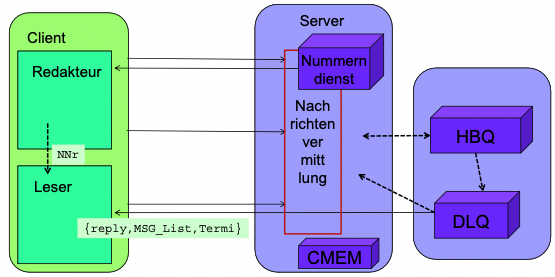
\includegraphics[scale=0.6]{Bilder/NachrichtendienstAbb.png}
\caption{\label{fig:nachrichtendienst} Nachrichtendienst \cite{Klauck2021}} 
\end{center}
\end{figure}

\subsection{Funktion der Holdback Queue}

Die Holdback Queue enthält alle Nachrichten, die nicht ausgeliefert werden dürfen. Das heißt, dass die enthaltenen Nachrichten nicht die richtigen Nummern für die Delivery Queue haben. Durch regelmäßiges Prüfen wird entschieden, ob inzwischen eine geeignete Nachricht für die Delivery Queue vom Server empfangen wurde. 

Da die Nachrichten nach aufsteigender Nummerierung an die Delivery Queue weitergeleitet werden, bietet es sich an diese in der Holdback Queue bereits zu sortieren. 
Um diese Sortierung möglichst effizient zu gestalten werden verschiedene Algorithmen getestet (siehe Kapitel \ref{Problemstellungen}.).

\subsection{Funktion der Delivery Queue}

Die Delivery Queue ist der abstrakte Speicher für alle Nachrichten, welche an den Client ausgeliefert werden können. Die Nachrichten sind innerhalb der Queue aufsteigend sortiert. Die eigentliche Schnittstelle zum Server ist aber trotzdem die Holdback Queue, da über diese die Nachrichten wieder versendet werden. Die Delivery Queue ist somit also lokal implementiert und wird von der Holdback Queue aufgerufen. 

\subsection{Aufbau der Nachrichten}

Nachrichten werden von den Redakteuren entwickelt und von den Lesern konsumiert. Bis sie beim Leser ankommen, können sie aber durch mögliche Software Fehler, wie z.B. asynchrone Nebenläufigkeiten oder ähnliches, verloren gehen. 
Die Nachrichten sind Tupel mit mindestens drei Elementen. Zum einen enthalten sie die Nachrichten-Nummer, nach welcher die Nachrichten sortiert werden. Dann enthalten sie eine Textzeile in welcher die eigentliche Nachricht geschrieben steht. Und abhängig davon, welche Queues sie schon durchlaufen haben, enthalten sie Zeitstempel mit den entsprechenden Eintritts- und Austrittszeiten. 

\subsection{Aufgabenerarbeitung}

Im Folgenden werden zuerst Entwürfe für die verschiedenen Queues mit ihren Funktionen erstellt, dabei wird vorerst nur die Implementierung der Holdback Queue als Heap und die Delivery Queue als Liste beschrieben. Die Entwürfe sollen nahe am zu implementierenden Code liegen, damit Fehler schnell eliminiert werden können. Um den Code zu testen werden Eunit Tests aus der Library 'eunit/include/eunit.hrl' geschrieben. Diese werden für spezifische Fälle angewendet, welche aus den Diagrammen der Entwürfe entschlossen werden können. So zum Beispiel der Fall, dass alle Elemente bei passender Nummerierung sofort von der Holdback zu der Delivery Queue weitergeleitet werden.
Nachdem die erste Version mit der Heapstruktur innerhalb der Holdback Queue funktioniert, wird eine zweite mit einer Listenstruktur implementiert. Diese beiden zu analysieren und zu vergleichen wird der Hauptbestandteil dieser Ausarbeitung sein. Zum Analysieren werden unter anderem die Benchmarks von Matz Heitmüller genutzt. Des Weiteren wird auch der Einfluss von Implementierungen mit Pattern Matching zu welchen mit if-else Statements verglichen. Nach diesem Teil wird ein Fazit erstellt in welchem die Messergebnisse ausgewertet werden. 

\subsection{Sortierung der Nachrichten} \label{Problemstellungen}

Problemstellung dieser Hausarbeit wird das Sortieren der Nachrichten innerhalb der Holdback Queue sein. Hierfür werden verschiedene Sortieralgorithmen getestet. Für verschiedene Algorithmen werden dann aber auch dementsprechend verschiedene abstrakte Datenstrukturen benötigt. So würde z.B. bei Insertion Sort nur das Konzept der Liste, also das 'Aneinander-pipen' von Elementen, reichen. Bei einem Heap Sort Algorithmus würde aber, wie der Name es schon andeutet, eine Heapstruktur verwendet werden müssen. Dieses Konzept basiert auf der Baumstruktur, es gibt also einen Wurzelknoten welcher einen linken und einen rechten Teilbaum haben kann.\\
Im vergangenen Praktikum 2 haben wir uns ausführlich mit Sortieralgorithmen befasst und drei bestimmte ausgewertet (siehe Abbildung \ref{fig:sortAlgo}). Aufsteigend, absteigend und random, bezieht sich hierbei auf die Liste welche sortiert wurde.

\begin{figure}[htbp]
\begin{center}
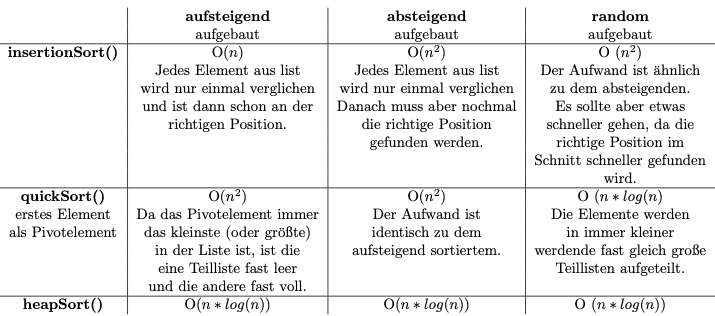
\includegraphics[scale=0.59]{Latex/Bilder/sortAlgo.png}
\caption{\label{fig:sortAlgo} Auswertung Sortieralgorithmen \cite{sortAlgo}} 
\end{center}
\end{figure}

Die bisherigen Algorithmen wurden aber bisher nur getestet, wenn mit statischen Listen gearbeitet wurde. Es also eine Liste übergeben wurde, diese fertig sortiert wird und dann mit dem nächsten Prozess begonnen wird. In dieser Anwendung wird allerdings dynamisch gearbeitet. Da der Holdback Queue ständig neue Nachrichten zugesendet werden, wäre ein Algorithmus geeignet, welcher im Online-Verfahren arbeitet. Er kennt also nicht alle Elemente welche zu sortieren sind, wenn er mit dem Sortieren beginnt. Interessant hierfür wäre also der InsertionSort Algorithmus. 
Wie es der bereitgestellten logging Datei "HB-DLQ@Qigong-KLC.log" (siehe Abb. \ref{fig:HBQFilesEntry2}) zu entnehmen ist, werden die Nachrichten von den Client-Servern der Redakteure mit sehr unbeständiger Nummerierung gesendet. Für den InsertionSort Algoithmus wäre dies aber ein Aufwand von O($n^2$). Im Folgenden wird ein dem InsertionSort ähnlicher Algorithmus verwendet. Im InsertionSort sucht ein Laufindex das nächste unsortierte Element und fügt es an der richtigen Stelle in der Liste ein. In diesem Anwendungsfall wäre der Laufindex immer an der Position null, da hier die neue Nachricht eingefügt wird. Dann wird der Index des Elements so lange erhöht, bis dieses die richtige Position erreicht hat. Wenn davon ausgegangen wird, dass die Elemente in zufälliger Reihenfolge eingefügt werden, entsteht eine Komplexität von $O(n/2)$. Beim Entfernen der Nachrichten gibt es in diesem Szenario den Vorteil, dass die Listen Erlang-intern mit dem ersten Element also Listenkopf (Head) beginnen und an diese die restliche Liste (Tail) angehängt wird. Somit kann beim Entfernen des kleinsten Elements mit dem Tail weitergearbeitet werden, was auf einen Aufwand von $O(1)$ schließen lässt.

\begin{figure}[htbp]
\begin{center}
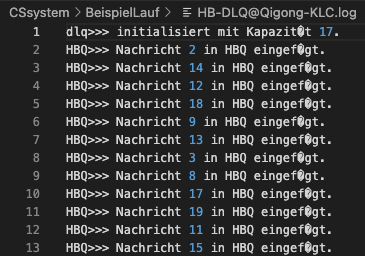
\includegraphics[scale=0.6]{Bilder/HBQFilesEntry.png}
\caption{\label{fig:HBQFilesEntry2} Nachrichtendienst \cite{HBQlogging}} 
\end{center}
\end{figure}

Der HeapSort Algorithmus an sich setzt eine Komplexität von $O(n*log(n))$ voraus. Das liegt daran, dass die zu sortierende Liste zuerst zu einem Heap umstrukturiert werden muss. Da dieser Schritt entfällt, angenommen man strukturiert diesen Heap von Anfang an, dann bleibt eine Komplexität von $O(log(n)$. Beachtet werden muss, dass der Aufwand beim Einfügen und beim Entfernen auch beim Heap nicht identisch ist. Beim Einfügen gilt $O(log(n))$, da das Element eventuell nur den Heap nach oben wandert. Beim Entfernen allerdings gilt $O(2*log(n))$, da hier das Wurzelelement nach dem Entfernen ersetzt wird und der Heap somit auch neu strukturiert werden muss. Der Heap Sortieralgorithmus ist also bei aufsteigend sortierter Liste mit O($3*log(n)$) leicht effizienter als der InsertionSort Algorithmus, allerdings mit gleichbleibender Effizienz deutlich besser bei random sortierter Liste. 

\subsection{Erwartungen} \label{erwartungen}

Das Ziel dieser Ausarbeitung ist es eine möglichst Effiziente Verarbeitung der Nachrichten zu erreichen. Der Fokus wird also auf der Sortierung der Elemente innerhalb der Holdback Queue, aber auch auf der Optimierung des allgemeinen Codes liegen.\\
Nach dem Vergleichen der beiden Implementierungen der Holdback Queue sollte die Sortierung über einen Heap als effizienter hervorgehen.\\
Außerdem wird vermutet, dass auch das Auslagern von Funktionen eine höhere Laufzeit zur Folge hat. Deswegen wird in einer Implementierung mit Hilfsfunktionen gearbeitet und in einer anderen auf diese verzichtet, was aber in einer teilweise sehr tiefen Codestruktur und einer dementsprechend schlechten Lesbarkeit resultieren wird. 
